\documentclass[10pt, twocolumn, a4paper]{article}
\usepackage[russian, english]{babel} % установка языков
\usepackage{graphicx} % вставка изображений
\usepackage{multicol} % деление на колонки
\usepackage{fancyhdr} % настройка колонтитулов
\usepackage{parskip} % настройка отступов абзаца
\usepackage{mathptmx} % Times New Roman
\usepackage{indentfirst} % отступ после заголовка секции
\usepackage{float} % плавающие картинки
\usepackage{titlesec} % настройка заголовков
\usepackage{setspace}
\usepackage[margin=0.1cm]{caption} % настройка описаний
\captionsetup[figure]{font=scriptsize} % шрифт описания фигуры
\usepackage[left=2.5cm,right=2cm, top=1cm,bottom=2.5cm]{geometry} % макет страницы
\fancyhf{} % очистка колонтитулов
\fancyfoot[C]{\textbf{\thepage}} % жирные номера страниц
\pagestyle{fancy}
\renewcommand{\headrulewidth}{0pt} % удаление линии header
\linespread{1.16} % межстрочный интервал
\setlength{\columnsep}{0.6cm} % расстояние между столбцами
\setlength{\parskip}{0pt} % вертикальный отступ абзаца
\setlength{\parindent}{0.5cm} % горизонтальный отступ абзаца
\setlength{\textfloatsep}{\theintvl\curtextsize} % отступ после картинок
\setcounter{page}{285} % нумерация страниц
\setcounter{figure}{1} % начальное значение нумерации фигур
\titleformat{\section}{\normalsize\centering}{\thesection. }{0cm}{}[] % стиль заголовков разделов
\titlespacing*{\section} % отступ возле секций
{0pt}{0cm}{0cm}
\renewcommand{\thesection}{\Roman{section}} % римские цифры
\setcounter{section}{0} % нумерация секций

\title{\textbf{Thyroid Gland Ultrasonography Automation\\
Through Intelligent Analysis}}
\author{Alena Cherkas\\\textit{Belarusian State University of}\\ \textit{Informatics and Radioelectronics}\\Minsk, Belarus\\Email: alena\_cherkas\_13@mail.ru}
\date{}

\begin{document}
\maketitle

\begin{spacing}{0.7}\textbf{\textit{Abstract}—This article proposes an algorithm for automating the process of medical ultrasound diagnostics using intelligent analysis. The actions are described using the example of a thyroid gland study. Additional verification of the result by the artificial intelligence allows novice doctors to feel more confident and minimize the influence of the human factor on the quality of diagnosis.}

\textbf{\textit{Keywords}—Ultrasonography automation; thyroid gland ultrasonography; artificial intelligence in medicine; intelligent image analysis; neural networks; deep learning; convolutional neural network; OSTIS; OSTIS Technology integration;}
\end{spacing}

\section{Introduction}

Currently, thyroid problems are widespread in the population of the Republic of Belarus. This is due to the disaster at the Chernobyl nuclear power plant in 1986. The Gomel and Mogilev regions of the country were the most affected. In the first 10 days after the accident, the concentration of radioactive iodine was increased in some territories of the republic, which led to an increase in cases of thyroid pathology.

According to the Ministry of Health for 2021, 3.8\% of the population of Belarus has pathology of this organ. There is an increase in the incidence every year.

Therefore, improving the technique of ultrasound diagnostics of thyroid pathologies is an urgent issue of our time.

Neural networks are gaining more and more popularity. They are often used in medical diagnostics. For example, to process test results, improve the quality of magnetic resonance imaging, analyze large amounts of data, and even perform surgical interventions.

By connecting artificial intelligence to the research, it is possible to reduce the influence of the human factor on the quality of the diagnosis. The result of ultrasound often depends on the doctor’s experience. After all, this type of diagnosis involves processing the results directly at the time of the study.

\section{Domain analysis}
Diagnostic ultrasound is a safe, non-invasive diagnostic technique used to image inside the body. Ultrasound
\begin{figure}[h!]
    \centering
    \includegraphics[width=1\linewidth, height=11cm]{heart.jpg}
    \caption{Thyroid gland scheme [1]}
    \label{fig:figure1}
\end{figure}
probes, called transducers, produce sound waves that have frequencies above the threshold of human hearing (above 20KHz), but most transducers in current use operate at much higher frequencies (in the megahertz (MHz) range).

Ultrasound waves are produced by a transducer, which can both emit ultrasound waves, as well as detect the ultrasound echoes reflected back. In most cases, the active elements in ultrasound transducers are made of special ceramic crystal materials called piezoelectrics. These materials are able to produce sound waves when an electric field is applied to them, but can also work in reverse, producing an electric field when a sound wave hits them. When used in an ultrasound scanner, the transducer sends out a beam of sound waves into the body.

The sound waves are reflected back to the transducer by boundaries between tissues in the path of the beam (e.g. the boundary between fluid and soft tissue or tissue and bone). When these echoes hit the transducer, they generate electrical signals that are sent to the ultrasound scanner. Using the speed of sound and the time of each echo’s return, the scanner calculates the distance from the transducer to the tissue boundary. These distances are then used to generate two-dimensional images of tissues and organs.

\begin{figure}[h!]
    \centering
    \includegraphics[width=1\linewidth]{comp.jpg}
    \caption{Ultrasound system scheme [2]}
    \label{fig:figure2}
\end{figure}

During an ultrasound exam, the technician will apply a gel to the skin. This keeps air pockets from forming between the transducer and the skin, which can block ultrasound waves from passing into the body. [3]

Ultrasound is a method of shadows. This study does not show a volumetric model of human organs, however, it allows to estimate the size, volume, density, correct location of the organ relative to the entire body, the presence of fluid in the area under study, as well as cysts, tumors and other formations. Moreover, minimally invasive operations are also performed under the control of an ultrasonic sensor. This allows the doctor to monitor the progress of the study without having to make large incisions on the human body.

During the ultrasound examination, the signal passes through the tissues of the human body and returns back. Solid dense organs reflect the sound signal well. Therefore, areas such as bones and stones look white on ultrasound.

Internal organs and soft tissues are usually represented by different shades of gray depending on the density of the organ.

Voids and liquid are shown in black on the screen, because in this case there are no obstacles in the signal path, and therefore it is practically not reflected at all.

Depending on the diagnostic areas, different types of sensors are used. The linear sensor has a rectangular image. The 2D sensor has a wide aperture, and its central frequency is in the range of 2.5-12 MHz (3D-4D is in the range of 7.5-11 MHz). Piezoelectric crystals in a linear sensor are located in the same plane, so such a sensor provides good visibility at close range. It is used for ultrasound of blood vessels, muscles, performing anesthesia under ultrasound control, examining mammary glands, thyroid gland and other superficial organs.

\begin{figure}[h!]
    \centering
    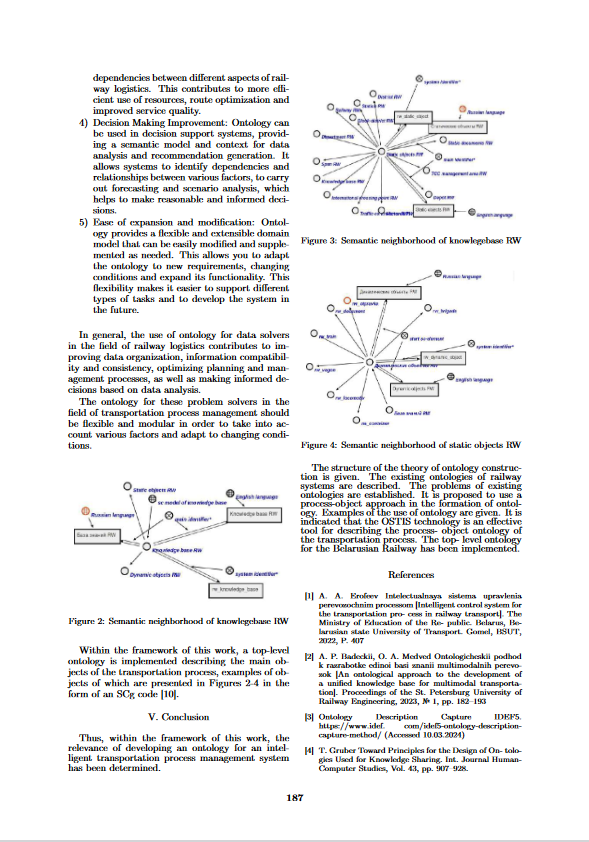
\includegraphics[width=1\linewidth]{pic3.jpg}
    \caption{An example of an ultrasound made by a linear sensor [4]}
    \label{fig:figure3}
\end{figure}

In a convex sensor, piezoelectric crystals are arranged curvilinearly. Therefore, such a sensor visualizes deeply located structures well. The convexic 2D sensor has a wide aperture, and its central frequency is 2.5-7.5 MHz (3D, 4D — 3.5-6.5 MHz). With its help, ultrasound of the fetus, pelvic organs, and abdominal cavity is performed.

The sector phased array sensor is so named after the type of piezoelectric element device, which is called a phased array. The phased array sensor has a small aperture and a low frequency (the central frequency is 2-7.5 MHz). The shape of the scanning area is almost triangular. These sensors have poor resolution in the near field but give a good view at depth. They allow to observe structures through a narrow intercostal gap. With its help, ultrasound of the heart, abdominal organs, and brain is performed.

For ultrasound diagnosis of the thyroid gland, only a linear sensor is often used. However, it is possible to see a trapezoidal image on the screen of the device. This is due to the fact that the linear sensor has the function of a virtual convection, which allows to make the viewing plane wider and accommodate the entire organ there.

The convex sensor is used only when the thyroid gland is enlarged and the patient’s body weight is too large.

Also ultrasound information can be displayed in several ways:

A-mode: As spikes on a graph (used to scan the eye).

B-mode: As a 2-dimensional anatomic images (used during pregnancy to evaluate the developing fetus or to evaluate internal organs).

\begin{figure}[h!]
    \centering
    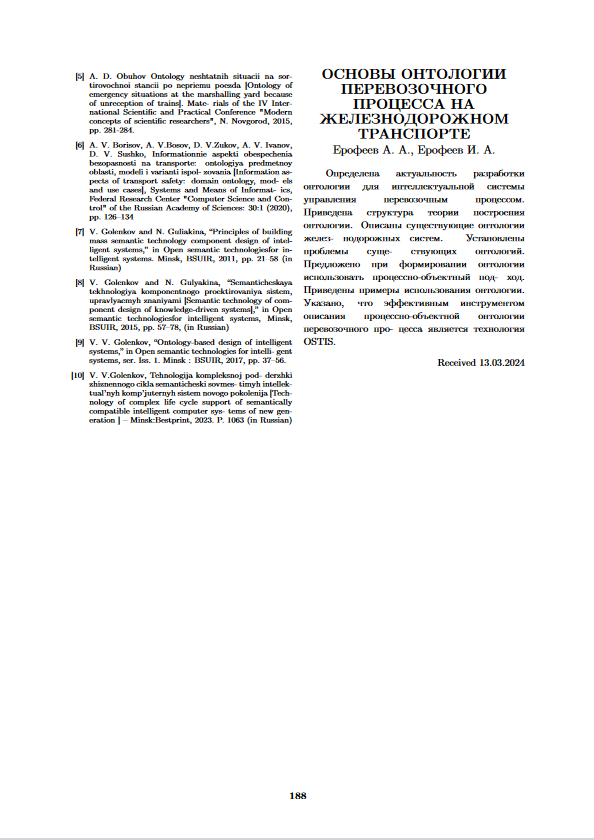
\includegraphics[width=1\linewidth]{pic4.jpg}
    \caption{An example of an ultrasound made by a linear sensor with virtual convex mode [5]}
    \label{fig:figure4}
\end{figure}

M-mode: As waves displayed continuously to show moving structures (used to evaluate the fetus’s heartbeat or to evaluate heart valve disorders).

B-mode ultrasonography is most commonly done. Sonography can be enhanced with Doppler measurements, which employ the Doppler effect to assess whether structures (usually blood) are moving towards or away from the probe, and its relative velocity. By calculating the frequency shift of a particular sample volume, for example a jet of blood flow over a heart valve, its speed and direction can be determined and visualised. This is particularly useful in cardiovascular studies (sonography of the vasculature system and heart) and essential in many areas such as determining reverse blood flow in the liver vasculature in portal hypertension. The Doppler information is displayed graphically using spectral Doppler, or as an image using color Doppler (directional Doppler) or power Doppler (non directional Doppler). This Doppler shift falls in the audible range and is often presented audibly using stereo speakers: this produces a very distinctive, although synthetic, pulsing sound.

Doppler ultrasonography uses changes that occur in the frequency of sound waves when they are reflected from a moving object (called the Doppler effect). In medical imaging, the moving objects are red blood cells in the blood. Thus, Doppler ultrasonography can be used to evaluate.

It is used to evaluate how well the heart is functioning (as part of echocardiography), to detect blocked blood vessels, especially in leg veins, as in deep vein thrombosis, when veins are blocked by a blood clot. To detect narrowed arteries, especially the carotid arteries in the neck, which carry blood to the brain.

Strictly speaking, most modern sonographic machines do not use the Doppler effect to measure velocity, as they rely on pulsed wave Doppler (PW). Pulsed wave machines transmit pulses of ultrasound, and then switch to receive mode. As such, the reflected pulse that they receive is not subject to a frequency shift, as the insonation is not continuous. However, by making several measurements, the phase change in subsequent measurements can be used to obtain the frequency shift (since frequency is the rate of change of phase). To obtain the phase shift between the received and transmitted signals, one of two algorithms is typically used: the Kasai algorithm or crosscorrelation. Older machines, that use continuous wave (CW) Doppler, exhibit the Doppler effect as described above. To do this, they must have separate transmission and reception transducers. The major drawback of CW machines, is that no distance information can be obtained (this is the major advantage of PW systems - the time between the transmitted and received pulses can be converted into a distance with knowledge of the speed of sound).

In the sonographic community (although not in the signal processing community), the terminology "Doppler" ultrasound, has been accepted to apply to both PW and CW Doppler systems despite the different mechanisms by which the velocity is measured.

Spectral Doppler ultrasonography shows blood flow information as a graph. It can be used to assess how much of a blood vessel is blocked.

\begin{figure}[h!]
    \centering
    
\includegraphics[width=1\linewidth]{pic5.jpg}
    \caption{An example of thyroid dopplerography [6]}
    \label{fig:figure5}
\end{figure}

\section{Overview of existing approaches}
There are already a lot of scientific articles on the processing of ultrasound results using artificial intelligence. Some of them are even applied in practice. Moreover, there is a S-Detect (Samsung RS80A ultrasound system, Seoul, Korea). It is the first commercially available ultrasound CAD based on deep learning technology for thyroid imaging. [7]

S-Detect is a computer-aided detection (CAD) software developed by Samsung Electronics for use with their RS80A ultrasound system. It is designed to assist
\newpage
\end{document}